
\chapter{Inference on Distributional Data \label{chap:EM}}

In this chapter, we formalize the problem of inference on distributional
data, and develop a novel Monte Carlo expectation-maximization algorithm
to conduct inference on such data.


\section{Stating and Formalizing the Problem}

We present in this section a generalization, stated informally in
\chapref{Introduction}, of the problem of inference on discretely
observed data from diffusion processes.


\subsection{The Discretely Observed Data Problem}

To begin, we review the problem of inference on diffusion processes
observed at discrete points in time. This is a topic of interest for
many statisticians, in large part due to the prevalence of diffusion
processes in modeling a wide range of phenomena, and the simultaneous
unavailability of continuous observations from such processes in the
real world. Consider a solution to the SDE
\begin{equation}
dX_{t}=\mu_{\theta}(X_{t})dt+\sigma_{\theta}(X_{t})dW_{t},\label{eq:sde-with-theta}
\end{equation}
where $\theta\in\Theta\subseteq\mathcal{R}^{p}$ is an unknown parameter
vector, $W$ is a Wiener process, and $\mu_{\theta}$ and $\sigma_{\theta}$
have known parametric forms up to $\theta$. Let $\mathcal{X}\subseteq\mathcal{R}$
be the state space of $X$. Suppose that we observe fixed values $\bar{\mathbf{x}}=\{\bar{x}_{t_{1}},\dots,\bar{x}_{t_{n}}\}\in\mathcal{X}^{n}$
at a collection of times $\mathcal{T}=\{t_{1}<\cdots<t_{n}=1\}$ where
$t_{1}>0$. Then, the log-likelihood of the data $\bar{\mathbf{x}}$
is 
\[
\ell(\theta\mid\bar{\mathbf{x}})=\sum_{i=1}^{n}\ell_{i}(\theta),
\]
where $\ell_{i}(\theta)=\log p_{\theta,t_{i}-t_{i-1}}(\bar{x}_{t_{i-1}},\bar{x}_{t_{i}})$
and $p_{\theta,t}(x,y)$ is the transition density associated with
(\ref{eq:sde-with-theta}) as usual (we assume $X_{t_{0}}=x_{0}$
is fixed). For many specifications of $\mu_{\theta}$ and $\sigma_{\theta}$,
$p_{\theta,t}(x,y)$ is not analytically tractable, and thus likelihood-based
inference on discretely observed data has historically been understood
to be quite difficult. In particular, maximum likelihood estimation
(MLE) has received significant attention in the literature, with proposed
approaches ranging from \citet{sahalia-2002}'s closed-form analytic
likelihood approximations to the simulation-based strategies of \citet{pedersen-1995}
and \citet{durham-gallant-2002}, and more recently, to imputation-based
techniques advanced by \citet{beskos-2006}. \citet{sorensen-2004}
offers a comprehensive survey of the range of inferential techniques
used for the problem of discretely observed diffusions.


\subsection{From Ex-Post to Ex-Ante}

We now present the central problem of this thesis. We can re-interpret
the discretely observed data problem by supposing we lived at $t_{0}=0$,
and viewing the data $\bar{\mathbf{x}}$ not as values of $X$ that
have already been observed, but rather as values that $X$ will take
on with certainty at future times $\mathcal{T}$ (perhaps as prophesized
by an omniscient Oracle). Modulo philosophical and measure-theoretic
subtleties, the problem has not changed materially: We ought to be
able to conduct likelihood-based inference using $\ell(\theta\mid\bar{\mathbf{x}}),$
so long as it is available, as usual.

This ex-ante perspective allows, however, for the generalization of
interest to this thesis. For we may suppose that instead of knowing
the values of $X$ at times $\mathcal{T}$, we know instead the joint
distribution $\nu$ of these values. Intuitively, knowing $\nu$ ought
to reveal information that we may use to learn about the parameters
governing the dynamics of $X$; on the other hand, the likelihood
function is no longer well-defined, and how to proceed with likelihood-based
inference is therefore unclear. We refer to $\nu$ as distributional
data, in juxtaposition with the observed data that is given in the
context of MLE.

The problems of inference on discretely observed data and on distributional
data are visualized in \figref{mle-intuition}. The fixed data depicted
on the left should help us learn about the dynamics of $X$ through
MLE (for instance, the data looks as if it contains some information
about the drift of $X$). The distributional data on the right, then,
with marginals centered at the fixed data, should contain at least
as much information about the dynamics of $X$, if not more.

\begin{figure}
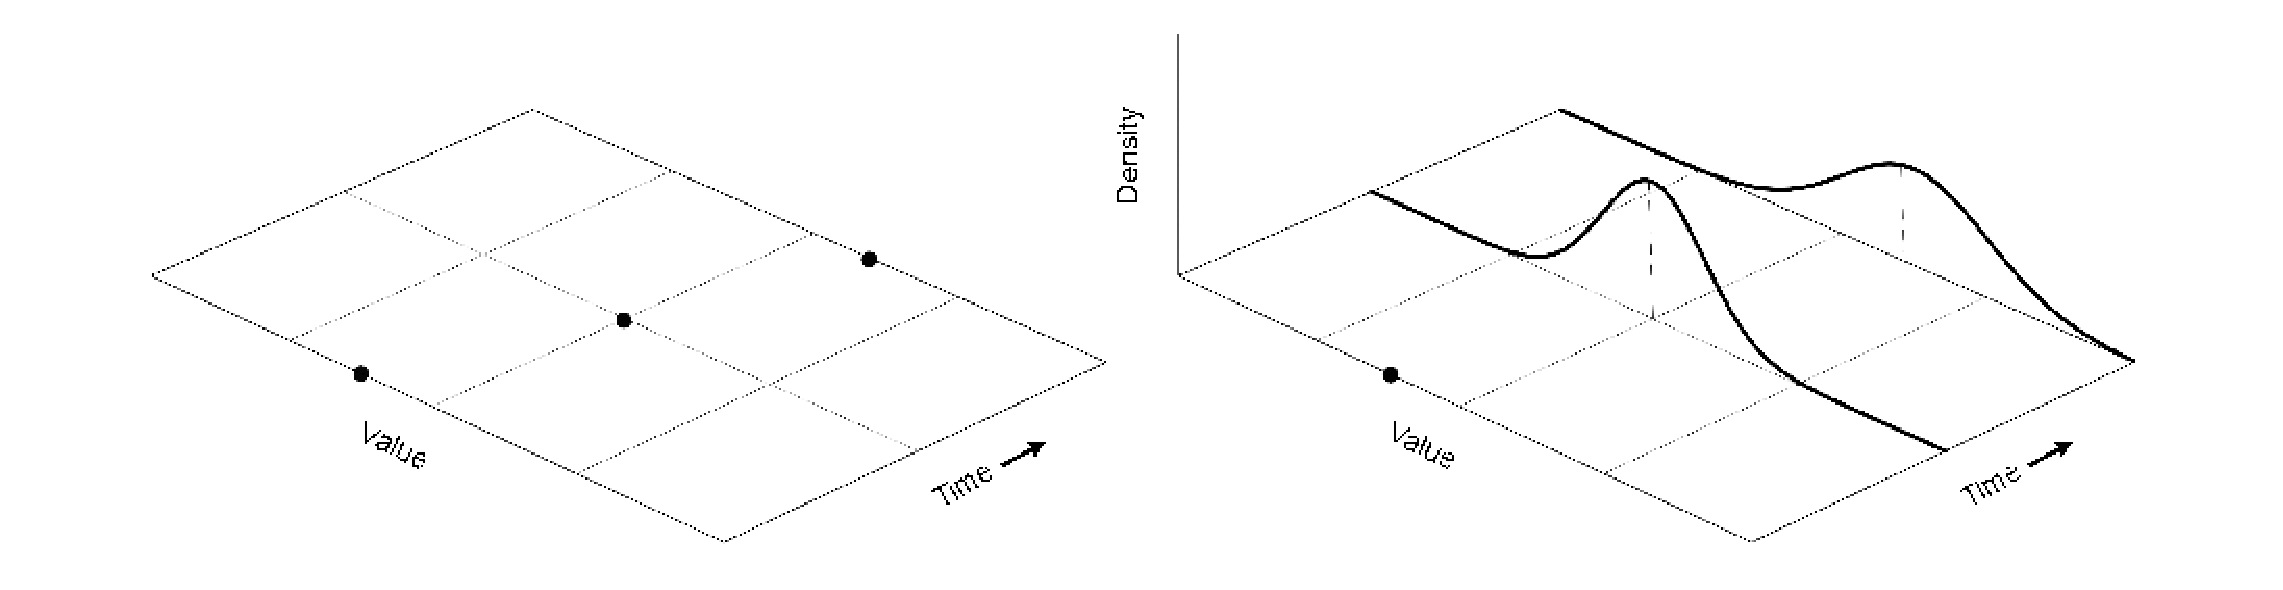
\includegraphics[width=1\columnwidth]{/Users/marshall/Documents/senior/thesis/figures/mle_vs_gen_ed}

\caption{\label{fig:mle-intuition}A visualization of the generalization of
MLE on discretely observed data proposed in this thesis. The value
of the process of interest at $t_{0}$ is fixed and indicated by a
black dot on the value axis. The left graphic depicts a fixed set
of data $\bar{\mathbf{x}}$ over time, on which MLE can be performed
if the log-likelihood is available. The right graphic depicts the
marginal distributions of a set of distributional data, where the
marginal distributions are centered at $\bar{\mathbf{x}}$.}
\end{figure}


In the remainder of this chapter, we will consider the identifiable
family of probability measures $\mathscr{\mathcal{Q}}=\{\mathbb{Q}_{\theta}\mid\theta\in\Theta\}$
on the usual probability space induced by solutions to (\ref{eq:sde-with-theta})
with some fixed initial condition $X_{0}=x_{0}$. We let $\mathbb{Q}_{\theta,X_{\mathcal{T}}}$
be the law of $X_{\mathcal{T}}$ under $\mathbb{Q}_{\theta}$ with
density $Q_{\theta,\mathcal{T}}$, and $\nu$ be an $n$-dimensional
distribution on the usual probability space restricted to times $\mathcal{T}$,
which is absolutely continuous to $\mathbb{Q}_{\theta,X_{\mathcal{T}}}$
for all $\theta\in\Theta$. Then, the problem of inference on distributional
data can loosely be stated as: What, if anything, can we say about
$\theta$, given $X_{\mathcal{T}}\sim\nu$?


\subsection{Proposing and Characterizing an Estimator}

In this subsection, we propose an estimator for $\theta$ given $X_{\mathcal{T}}\sim\nu$,
and make some remarks characterizing its relationship to the maximum
likelihood estimator given discretely observed data.

We first note that from the ex-ante perspective presented above, the
problem of discretely observed data is a special case of the problem
of distributional data. Intuitively, if we were given distributional
data under which $X_{\mathcal{T}}$ was a degenerate random variable,
we would know the values that $X$ would take on with certainty at
future times $\mathcal{T}$ (again, modulo philosophical and measure-theoretic
subtleties). Then, the problem of distributional data could be solved
through traditional MLE. Slightly more formally, we can fix some data
$\bar{\mathbf{x}}\in\mathcal{X}^{n}$. If $\{\nu_{(m)}\}$ is a sequence
of probability measures which are absolutely continuous to $\mathbb{Q}_{\theta,X_{\mathcal{T}}}$
and which converge (in some sense) to the Dirac delta measure $\delta_{\bar{\mathbf{x}}}$,
then as $m\rightarrow\infty$, any estimator for $\theta$ given $X_{\mathcal{T}}\sim\nu_{(m)}$
should coincide with the MLE given $\bar{\mathbf{x}}$. A quantity
that should satisfy this criterion is 
\begin{equation}
\arg\max_{\theta\in\Theta}\int\log Q_{\theta,\mathcal{T}}(x)\nu(dx).\label{eq:mklde}
\end{equation}


We define $\Lambda_{\theta}(\nu)\coloneqq\int\log Q_{\theta,\mathcal{T}}(x)\nu(dx)$,
alluding with our notation to the traditional log-likelihood function
$\ell_{\theta}(\bar{\mathbf{x}})$. We note that $\arg\max_{\theta\in\Theta}\Lambda_{\theta}(\nu)$
is not an estimator in the technical sense since it is a functional
of a distribution $\nu$, rather than a function of observed data.
In this thesis, we will use the term ``estimator'' loosely to refer
to any function(al) of data (distributional or otherwise) that is
used to infer the value of an unknown parameter in a statistical model. 

As \citet[Section 1 in][]{akaike-1973} notes, maximizing $\Lambda_{\theta}(\nu)$
is equivalent to minimizing the K-L divergence of $\mathbb{Q}_{\theta,X_{\mathcal{T}}}$
from $\nu$. This is easily seen by writing 
\begin{eqnarray*}
D(\nu\:||\:\mathbb{Q}_{\theta,X_{\mathcal{T}}}) & = & \mathbb{E}_{\nu}\left[\log\frac{d\nu}{d\mathbb{Q}_{\theta,X_{\mathcal{T}}}}\right]\\
 & = & \mathbb{E}_{\nu}\left[\log\frac{d\nu}{dx}\right]-\mathbb{E}_{\nu}\left[\log\frac{d\mathbb{Q}_{\theta,X_{\mathcal{T}}}}{dx}\right].
\end{eqnarray*}


For this reason, we call the proposed estimator for $\theta$ in (\ref{eq:mklde})
the minimum K-L divergence estimator (MKLDE) given $\nu$. We now
present two remarks, which
\begin{aenumerate}
\item characterize the MKLDE given $\nu$ as a limiting case of maximum
likelihood estimation under model misspecification when $\nu$ is
a true probability model, and
\item show that a (traditional) estimator given finitely many samples from
$\nu$ asymptotically converges to the MKLDE given $\nu$.
\end{aenumerate}
The first remark connects the MKLDE given $\nu$ to the MLE under
model misspecification.
\begin{rem}
\label{rem:misspecification}Let $\nu$ be the true distribution of
$X$ at times $\mathcal{T}$, and consider $N$ i.i.d draws from $\nu$,
$\{X_{\mathcal{T},(i)}\}_{i=1,\dots,N}$. If we wished to model $\nu$
using the family of potentially misspecified probability models $\mathcal{Q}$
restricted to $\mathcal{T}$, the MLE given $\{X_{\mathcal{T},(i)}\}_{i=1,\dots,N}$
would be 
\[
\arg\max_{\theta\in\Theta}\frac{1}{N}\sum_{i=1}^{N}\log Q_{\theta,\mathcal{T}}(X_{\mathcal{T},(i)}).
\]
By a result of \citet[Theorem 2.2 in][]{white-1982}, 
\[
\arg\max_{\theta\in\Theta}\frac{1}{N}\sum_{i=1}^{N}\log Q_{\theta,\mathcal{T}}(X_{\mathcal{T},(i)})\xrightarrow{p}\arg\min_{\theta\in\Theta}\mathbb{E}_{\nu}\left[\log\frac{d\nu}{d\mathbb{Q}_{\theta,X_{\mathcal{T}}}}\right]
\]
as $N\rightarrow\infty$, and thus by the observation of \citet{akaike-1973},
\[
\arg\max_{\theta\in\Theta}\frac{1}{N}\sum_{i=1}^{N}\log Q_{\theta,\mathcal{T}}(X_{\mathcal{T},(i)})\xrightarrow{p}\arg\max_{\theta\in\Theta}\Lambda_{\theta}(\nu),
\]
which is the MKLDE.
\end{rem}
The intuition for this relationship is as follows. Recall that a time-homogenous
Markov measure is uniquely determined by a transition kernel and a
marginal measure; an SDE satisfying the requirements outlined in \chapref{2}
along with the initial condition $X_{0}=x_{0}$ therefore admits a
bijection between $\Theta$ and $\mathcal{Q}$. Now suppose we know
$X_{\mathcal{T}}\sim\nu$. If $\nu$ is not the law of $X_{\mathcal{T}}$
under any element of $\mathcal{Q}$, it must be the case that we have
misspecified our probability model. In this case, the best we can
do is to find the value of $\theta$ that minimizes the K-L divergence
of $\mathbb{Q}_{\theta,X_{\mathcal{T}}}$ from $\nu$, which is precisely
the MKLDE given $\nu$.

In practice, we will often only have access to a finite number of
draws from $\nu$; think, for instance, of the forecasts for humidity
that a panel of finitely many weatherpeople might give. We now remark
on the consistency of the MKLDE given only a fixed number of samples
from $\nu$.
\begin{rem}
\label{rem:bootstrap}Let $\hat{\nu}_{(N)}$ be the empirical distribution
function induced by $N$ draws from $\nu$, and consider $N$ i.i.d
draws from $\hat{\nu}_{(N)}$, $\{X_{\mathcal{T},(i)}\}_{i=1,\dots,N}$.
By standard results demonstrating the consistency of plug-in bootstrap
estimators (see \citet[Section 1 in][]{horowitz-2002}), 
\begin{eqnarray*}
\Lambda_{\theta}(\hat{\nu}_{(N)}) & = & \int\log P_{\theta,\mathcal{T}}(x)\hat{\nu}_{(N)}(dx)\\
 & = & \frac{1}{N}\sum_{i=1}^{N}\log Q_{\theta,\mathcal{T}}(X_{\mathcal{T},(i)})\\
 & \xrightarrow{p} & \Lambda_{\theta}(\nu)
\end{eqnarray*}
and by a loose application of the $\arg\max$ continuous mapping theorem
(see \citet[Theorem 2.7 in][]{kim-pollard-1990}), 
\[
\arg\max_{\theta\in\Theta}\Lambda_{\theta}(\hat{\nu}_{(N)})\xrightarrow{p}\arg\max_{\theta\in\Theta}\Lambda_{\theta}(\nu),
\]
which is the MKLDE given $\nu$.
\end{rem}
This remark shows that an estimator for $\theta$ can be developed
when only given finitely many samples from $\nu$; we simply use the
empirical distribution of the samples as a plug-in estimate for $\nu$
in (\ref{eq:mklde}). This estimator is consistent for the true minimum
K-L divergence parameter, and is an estimator in the traditional technical
sense since $\hat{\nu}$, and by extension $\Lambda_{\theta}(\hat{\nu})$,
is a function of fixed observations. We will simply call this estimator
the MKLDE given $\hat{\nu}$, with the underlying data implicit, in
direct analogy to the MKLDE given $\nu$ defined in (\ref{eq:mklde}),
and refer to both these estimators more generally as the MKLDE.

Together, the two remarks presented above describe why (\ref{eq:mklde})
is statistically meaningful in the context of distributional data.
In particular, suppose $\mathbb{P}$ is a true but unknown probability
model, but the law of $X_{\mathcal{T}}$ under $\mathbb{P}$ is known
to be $\nu$. Then, the MKDLE given $\nu$ over any parameterized
family of probability models $\mathcal{Q}$ identifies the $\mathbb{Q}_{\theta}\in\mathcal{Q}$
such that $\mathbb{Q}_{\theta,X_{\mathcal{T}}}$ has the minimum K-L
divergence from $\nu$. The MKLDE is furthermore asymptotically consistent
when we use the empirical law of samples from $\nu$ as a plug-in
estimate for $\nu$.

While we have shown that the MKDLE is meaningful, given the unavailability
of a transition density for most diffusion processes, it is clear
that $\Lambda_{\theta}(\nu)$ has no obvious functional form for all
but the most specific choices of $\mu_{\theta},\sigma_{\theta}$,
and $\nu$. Solving for the MKLDE is therefore impossible from an
analytic standpoint; the next section addresses this issue by developing
a simulation-based strategy for finding the MKLDE.


\section{Simulation-Based K-L Divergence Minimization}

Simulation-based inference techniques have been applied widely in
the literature to solve the problem of likelihood-based inference
on discretely observed diffusions. This approach began with the seminal
paper of \citet{pedersen-1995}. More recently, \citet{roberts-stramer-2001,elerian-chib-shephard-2001},
and others simultaneously realized that the problem of discrete observations
could be framed in terms of missing data. In particular, though the
likelihood function given discrete observations is in general intractable,
Girsanov's formula can give the likelihood of the observations when
they are augmented with the continuous path of the process in question
between observations. \citet{beskos-2006}, building on techniques
developed by \citet{dempster-1977} and \citet{wei-tanner-1990},
show that the simulation of diffusion bridges (using the Exact Algorithm
of \citet{beskos-roberts-2005}) could be leveraged to supply this
missing data; this approach will be of particular interest to us.

In this section, we generalize the results of \citet{roberts-stramer-2001,beskos-2006},
and \citet{bladt-sorensen-2014} to propose a simulation-based method
to find the MKLDE. As noted above, $\Lambda_{\theta}(\nu)$ cannot
be maximized analytically. However, we use the close parallels between
the MLE given discretely observed data and the MKLDE given distributional
data to develop an MCEM algorithm which converges to $\arg\max_{\theta\in\Theta}\Lambda_{\theta}(\nu)$.


\subsection{The Case of Unit Diffusion Coefficient}

We will first consider the highly specific case of $\sigma_{\theta}(x)$
in (\ref{eq:sde-with-theta}) being equal to unity so that we may
focus deriving the general shape of a simulation strategy. In particular,
we prove the central result of this chapter in this subsection, which
gives a novel EM algorithm which maximizes $\Lambda_{\theta}(\nu)$
in a manner analagous to the EM algorithm of \citet[Section 8 in][]{beskos-2006},
which maximizes $\ell_{\theta}(\bar{\mathbf{x}})$ for discretely
observed data $\bar{\mathbf{x}}\in\mathcal{X}^{n}$.
\begin{thm}
\label{thm:em}Suppose $\sigma_{\theta}(x)=1$ in (\ref{eq:sde-with-theta}).
Then, let $\mathcal{Q}=\{\mathbb{Q}_{\theta}\mid\theta\in\Theta\}$
be the identifiable family of probability measures that are induced
by solutions to (\ref{eq:sde-with-theta}) with constant initial condition.
Fix a parameter estimate $\tilde{\theta}\in\Theta$ and let $\nu$
be a distribution satisfying the usual assumptions. If $\mathbb{Q}_{\tilde{\theta}}^{\nu}$
is the Baudoin $(X_{\mathcal{T}},\nu)$-conditioning of $\mathbb{Q}_{\tilde{\theta}}\in\mathcal{Q}$,
then 
\begin{equation}
\arg\max_{\theta\in\Theta}\Lambda_{\theta}(\nu)-\Lambda_{\tilde{\theta}}(\nu)=\arg\max_{\theta\in\Theta}\mathbb{E}_{\mathbb{Q}_{\tilde{\theta}}^{\nu}}\left[\int_{0}^{1}\mu_{\theta}(X_{s})dX_{s}-\frac{1}{2}\int_{0}^{1}\mu_{\theta}^{2}(X_{s})ds\right].\label{eq:em-equation}
\end{equation}
gives an iteration of an EM algorithm which converges to the MKLDE
given $\nu$. In particular, repeated iterations of (\ref{eq:em-equation})
converge to the parameter $\theta^{*}\in\Theta$ such that the law
of $X_{\mathcal{T}}$ under $\mathbb{Q}_{\theta^{*}}$ has the minimum
K-L divergence from $\nu$, for any $\mathbb{Q}_{\theta}\in\mathcal{Q}$.\end{thm}
\begin{proof}
We begin by re-expressing the objective function on the left hand
side of (\ref{eq:em-equation}) as 
\begin{eqnarray}
\Lambda_{\theta}(\nu)-\Lambda_{\tilde{\theta}}(\nu) & = & \int\log Q_{\theta,\mathcal{T}}(x_{\mathcal{T}})\nu(dx_{\mathcal{T}})-\Lambda_{\tilde{\theta}}(\nu)\nonumber \\
 & = & \int\log\int Q_{\theta,\mathcal{T}}(x_{\mathcal{T}}\mid x)Q_{\theta}(x)dx\nu(dx_{\mathcal{T}})-\Lambda_{\tilde{\theta}}(\nu),\label{eq:firststepem}
\end{eqnarray}
where we take\textbf{ $X$ }to be missing data representing the path
of a solution to (\ref{eq:sde-with-theta}) on $[0,1]$. Then, in
a similar fashion to standard arguments in the derivation of the EM
algorithm (see, for instance, \citet[Section 3.1 in][]{borman-2006}),
we can find from (\ref{eq:firststepem}) that

\begin{align}
\Lambda_{\theta}(\nu)-\Lambda_{\tilde{\theta}}(\nu) & \geq\iint\log\left(\frac{Q_{\theta,\mathcal{T}}(x_{\mathcal{T}}\mid x)Q_{\theta}(x)}{Q_{\tilde{\theta}}(x\mid x_{\mathcal{T}})}\right)P_{\tilde{\theta}}(x\mid x_{\mathcal{T}})dx\nu(dx_{\mathcal{T}})-\Lambda_{\tilde{\theta}}(\nu)\nonumber \\
 & =\iint\log\left(\frac{Q_{\theta,\mathcal{T}}(x_{\mathcal{T}}\mid x)Q_{\theta}(x)}{Q_{\tilde{\theta}}(x\mid x_{\mathcal{T}})Q_{\tilde{\theta},\mathcal{T}}(x_{\mathcal{T}})}\right)P_{\tilde{\theta}}(x\mid x_{\mathcal{T}})dx\nu(dx_{\mathcal{T}}).\label{eq:Deltatn}
\end{align}
We define the quantity in (\ref{eq:Deltatn}) as $\Delta(\theta\mid\tilde{\theta})$,
and let $\mathscr{Q}(\theta\mid\tilde{\theta})\coloneqq\Lambda_{\tilde{\theta}}(\nu)+\Delta(\theta\mid\tilde{\theta})\leq\Lambda_{\theta}(\nu)$.
It can be shown by standard arguments that $\mathscr{Q}(\tilde{\theta}\mid\tilde{\theta})=\Lambda_{\tilde{\theta}}(\nu$),
and so any $\theta$ that increases $\mathscr{Q}(\theta\mid\tilde{\theta})$
must also increase $\Lambda^{\nu}(\theta)$. To maximize this increase,
it suffices to solve for
\begin{eqnarray*}
\arg\max_{\theta\in\Theta}\mathscr{Q}(\theta\mid\tilde{\theta}) & = & \arg\max_{\theta\in\Theta}\iint\log\left(\frac{Q_{\theta,\mathcal{T}}(x_{\mathcal{T}}\mid x)Q_{\theta}(x)}{Q_{\tilde{\theta}}(x\mid x_{\mathcal{T}})Q_{\tilde{\theta},\mathcal{T}}(x_{\mathcal{T}})}\right)Q_{\tilde{\theta}}(x\mid x_{\mathcal{T}})dx\nu(dx_{\mathcal{T}})\\
 & = & \arg\max_{\theta\in\Theta}\iint\log Q_{\theta}(x)Q_{\tilde{\theta}}(x\mid x_{\mathcal{T}})dx\nu(dx_{\mathcal{T}})\\
 & = & \arg\max_{\theta\in\Theta}\int\log Q_{\theta}(x)\mathbb{Q}_{\tilde{\theta}}^{\nu}(dx).
\end{eqnarray*}
The first equality follows from dropping terms that are constant with
respect to $\theta$, including $Q_{\theta,\mathcal{T}}(x_{\mathcal{T}}\mid x)$
since the full path $x$ is fixed. The second equality follows from
the assumption of some regularity conditions that allow for switching
the order of integration and the existence of the requisite densities,
and from the definition of a Baudoin conditioning.

By Girsanov's theorem, since the complete path $X$ has unit diffusion
coefficient, we may write 
\[
\log Q_{\theta}(X)=\int_{0}^{1}\mu_{\theta}(X_{s})dx_{s}-\frac{1}{2}\int_{0}^{1}\mu_{\theta}^{2}(X_{s})ds,
\]
and (\ref{eq:em-equation}) follows. As in any EM algorithm, repeated
iterations of $\tilde{\theta}=\arg\max_{\theta\in\Theta}Q(\theta\mid\tilde{\theta})$
will converge to $\arg\max_{\theta\in\Theta}\Lambda_{\theta}(\nu)$,
which is precisely the MKLDE.
\end{proof}
Note that when $\nu=\delta_{\bar{\mathbf{x}}}$ (in some limiting
sense) for fixed data $\bar{\mathbf{x}}$ observed at $\mathcal{T}$,
(\ref{eq:em-equation}) reduces to 
\[
\arg\max_{\theta\in\Theta}\ell(\theta\mid\bar{\mathbf{x}})-\ell(\tilde{\theta}\mid\bar{\mathbf{x}})=\arg\max_{\theta}\mathbb{E}_{X\mid\bar{\mathbf{x}},\tilde{\theta}}\left[\int_{0}^{1}\mu_{\theta}(X_{s})dX_{s}-\frac{1}{2}\int_{0}^{1}\mu_{\theta}^{2}(X_{s})ds\right]
\]
where the expectation is taken over traditional diffusion bridges
$X$ conditioned on $\bar{\mathbf{x}}$. This equation is simply the
EM algorithm of \citet{beskos-2006} for discretely observed data. 

Though (\ref{eq:em-equation}) is intractable, given the ability to
sample $X$ under $\mathbb{Q}_{\tilde{\theta}}^{\nu}$, it is suggestive
of a Monte Carlo implementation of the EM algorithm following \citet{wei-tanner-1990}.
But before developing such an implementation, we generalize (\ref{eq:em-equation})
for the case of diffusion coefficients known only up to $\theta$.


\subsection{Augmentation Under the Lamperti Transform}

The restriction of the diffusion coefficient to unity severely reduces
the utility of the EM algorithm in practical settings. In this subsection,
we relax this assumption and derive an EM algorithm suitable for general
use. Our general strategy to deal with a diffusion with general diffusion
coefficient is to first transform it into one with unit diffusion
coefficient. Then, after some further transformations, we can derive
the log-likelihood of such a transformed process using Girsanov's
theorem, and substitute this likelihood into (\ref{eq:em-equation}).

Recall that for any solution to (\ref{eq:sde-with-theta}), we may
define the Lamperti transform $\eta_{\theta}(x)$, where
\[
\eta_{\theta}(x)=\int_{x^{*}}^{x}\frac{1}{\sigma_{\theta}(y)}dy,
\]
for appropriate but otherwise arbitrary $x^{*}$. If we set $Y_{t}=\eta_{\theta}(X_{t})$,
by It�'s lemma, $Y$ is the solution to the stochastic differential
equation
\begin{equation}
dY_{t}=\alpha_{\theta}(Y_{t})dt+dW_{t},\label{eq:eta-y}
\end{equation}
where 
\[
\alpha_{\theta}(y)=\frac{\mu_{\theta}(\eta_{\theta}^{-1}(y))}{\sigma_{\theta}(\eta_{\theta}^{-1}(y))}-\frac{1}{2}\sigma_{\theta}^{'}(\eta_{\theta}^{-1}(y)).
\]
We use $\mathbb{Y}_{\theta}$ to denote the measure induced by a solution
to (\ref{eq:eta-y}) with constant initial condition $Y_{0}=\eta_{\theta}(x_{0}).$ 

(\ref{eq:eta-y}) reveals that the Lamperti transform is a continuous
transformation which reduces the diffusion coefficient of any diffusion
to unity. However, \citet{bladt-sorensen-2014} point out that under
the Lamperti transform, the distribution of $Y$ at times $\mathcal{T}$
becomes dependent on the parameter $\theta$, while the EM algorithm
requires that the given data remain fixed with respect to $\theta$.
We adapt their proposed solution to our problem, referring the reader
to \citet[Section 4.1 in][]{bladt-sorensen-2014}, who build on techniques
developed in \citet[Section 3.2 in][]{roberts-stramer-2001} and \citet[Section 8.2 in][]{beskos-2006},
for the theoretical details of the approach. 

Heuristically, our solution is to generate paths of $Y$ under $\tilde{\theta}$
and apply linear transformations to these paths so that they ``look''
like paths under $\theta$. In this way, for each iteration of the
EM algorithm, the given distributional data remains fixed with respect
to $\theta$. In particular, we consider $t_{i-1}\leq t\leq t_{i}$
for each $i=1,\dots,n$. Let $Z(\tilde{\theta})$ be a path under
$\mathbb{Y}_{\tilde{\theta}}^{\nu\circ\eta_{\tilde{\theta}}^{-1}}\eqqcolon\mathbb{Z}_{\tilde{\theta}}$
i.e. a solution to (\ref{eq:eta-y}) conditioned to follow the distribution
$\nu\circ\eta_{\tilde{\theta}}^{-1}$ at times $\mathcal{T}$. Setting
$H_{\tilde{\theta}\rightarrow\theta}=\eta_{\theta}\circ\eta_{\tilde{\theta}}^{-1}$,
we define 
\begin{eqnarray*}
Y_{t}^{*}(\theta,\tilde{\theta}) & = & Z_{t}(\tilde{\theta})+\frac{(t_{i}-t)(H_{\tilde{\theta}\rightarrow\theta}(Z_{t_{i-1}}(\tilde{\theta}))-Z_{t_{i-1}}(\tilde{\theta}))}{t_{i}-t_{i-1}}+\\
 &  & \frac{(t-t_{i-1})(H_{\tilde{\theta}\rightarrow\theta}(Z_{t_{i}}(\tilde{\theta}))-Z_{t_{i}}(\tilde{\theta}))}{t_{i}-t_{i-1}}.
\end{eqnarray*}
Note that $Y_{t_{i-1}}^{*}(\theta,\tilde{\theta})=H_{\tilde{\theta}\rightarrow\theta}(Z_{t_{i-1}}(\tilde{\theta}))$
and $Y_{t_{i}}^{*}(\theta,\tilde{\theta})=H_{\tilde{\theta}\rightarrow\theta}(Z_{t_{i}}(\tilde{\theta}))$;
in this sense, $Y_{\mathcal{T}}^{*}$ ``looks'' like it is distributed
according to $\nu\circ\eta_{\theta}^{-1}$, though it is generated
using a path that is only governed by $\tilde{\theta}$. Now, we let
\begin{aenumerate}
\item $A_{\theta}(u)=\int_{u^{*}}^{u}\alpha_{\theta}$ for suitable but
otherwise arbitrary $u^{*}$, and
\item $\nu_{i,j,\dots}$ be the distribution of the $(i,j,\dots)$-th coordinates
of $\nu$
\end{aenumerate}
and use a result of \citet[Lemma 2 in][]{beskos-2006} to find the
conditional expectation of the continuous log-likelihood function
of $Y_{t}^{*}(\theta,\tilde{\theta})$: 
\begin{eqnarray}
\mathscr{Q}(\theta\mid\tilde{\theta}) & = & \mathbb{E}_{\nu_{n}}\left[A_{\theta}(\eta_{\theta}(X_{t_{n}}))\right]-A_{\theta}(\eta_{\theta}(x_{0}))-\nonumber \\
 &  & \sum_{i=1}^{n}\mathbb{E}_{\nu_{i}}\left[\log(\sigma_{\theta}(X_{t_{i}}))\right]-\nonumber \\
 &  & \frac{1}{2}\sum_{i=1}^{n}\mathbb{E}_{\nu_{i-1,i}}\left[(\eta_{\theta}(X_{t_{i}})-\eta_{\theta}(X_{t_{i-1}}))^{2}/(t_{i}-t_{i-1})\right]-\nonumber \\
 &  & \frac{1}{2}\mathbb{E}_{\mathbb{Z}_{\tilde{\theta}}}\left[\int_{0}^{1}\left(\alpha_{\theta}^{2}+\alpha_{\theta}^{'}\right)\left(Y_{s}^{*}(\theta,\tilde{\theta})\right)ds\right].\label{eq:final-q-1}
\end{eqnarray}


\begin{algorithm}
\caption{MCEM for the MKLDE Given Distributional Data $\nu$}


\begin{algorithmic}[1] 
\Function{$\mathscr{Q}$}{$\theta, \tilde{\theta}, \nu, N, M$}
	\State{$\mathscr{Q} \gets  $\Call{mean}{$A_{\theta}(\eta_{\theta}($\Call{sample}{$\nu, N$}$[,n]))$}}
	\State{$\mathscr{Q} \gets \mathscr{Q} \:-\: $\Call{mean}{$A_{\theta}(\eta_{\theta}($\Call{sample}{$\nu, N$}$[,1]))$}}
	\State{$\mathscr{Q} \gets \mathscr{Q} \:-\: $\Call{sum}{\Call{col-means}{$\log(\sigma_{\theta}($\Call{sample}{$\nu, N$}$)$}}}
	\State{$\mathscr{Q} \gets \mathscr{Q} \:-\: $\Call{sum}{\Call{col-means}{\Call{row-diffs}{$\eta_{\theta}($\Call{sample}{$\nu, N$}$)$}$^2}/$\Call{diff}{$\mathcal{T}$}}}
	\For{$t_i$ in $\mathcal{T}$}
		\State{$S_i \gets 0, \Delta \gets t_i - t_{i-1}, \delta \gets \Delta / M$}
		\For{$N$ iterations}
			\State{\textbf{sample} $t$ from $\{0,\delta,\dots,M\delta\}$}
			\State{$\mathbf{Z} \gets$ \Call{exact baudoin-bridge}{$\alpha_{\tilde{\theta}},1,\nu_{i-1,i} \circ \eta_{\tilde{\theta}}^{-1}, M, \Delta$}}
			\State{$Y^{*}_t \gets \mathbf{Z}_{t} + \Delta^{-1}((t_i - t)(H_{\tilde{\theta} \rightarrow \theta} (\mathbf{Z}_0) - \mathbf{Z}_0) + (t-t_{i-1})(H_{\tilde{\theta}\rightarrow\theta}(\mathbf{Z}_\Delta) - \mathbf{Z}_\Delta))$}
			\State{$S_i \gets S_i + (\alpha_{\theta}^2 + \alpha_{\theta}^{'})(Y^{*}_t)/N$}
		\EndFor
		\State{$\mathscr{Q} \gets Q \:-\:\frac{\Delta}{2}S_i$} 
	\EndFor
	\State \Return{$\mathscr{Q}$}
\EndFunction

\Function{find-mklde}{$\theta_0, \nu, N, M$}
	\State{$\tilde{\theta} \gets \theta_0$}
	\Repeat	
	\State{$\tilde{\theta} = \arg \max_{\theta \in \Theta} \mathscr{Q}(\theta, \tilde{\theta}, \nu, N, M)$}
	\Until{convergence}
	\State \Return{$\tilde{\theta}$}
\EndFunction

\end{algorithmic}

\label{algo:mcem}
\end{algorithm}


Note that by standard Monte Carlo integration results, we may re-write
the last term in (\ref{eq:final-q-1}) as 
\[
\frac{1}{2}\mathbb{E}_{\mathbb{Z}_{\tilde{\theta}},U}\left[\left(\alpha_{\theta}^{2}+\alpha_{\theta}^{'}\right)\left(Y_{U}^{*}(\theta,\tilde{\theta})\right)\right]
\]
for some independent $U\sim\mbox{Unif}[0,1]$. 

While (\ref{eq:final-q-1}) remains hopelessly intractable, it immediately
suggests a MCEM scheme, assuming we have a way of sampling paths under
Baudoin bridge measures. Suppose for the moment we do: the function
\noun{exact baudoin-bridge}(\textbf{\noun{$\mu,\sigma,\nu,M,\Delta$}})
will return discrete observations $\mathbf{X}=\{\mathbf{X}_{t}\}_{t=0,\delta,\dots,M\delta}$
for $\delta=\Delta/M$ of an It� diffusion with drift coefficient
$\mu(x)$ and diffusion coefficient $\sigma(x)$ under the Baudoin
$(X_{0,\Delta},\nu)$-conditioning of its associated measure on $[0,\Delta]$,
where $\Delta\in(0,1]$. Further suppose we have a function \noun{sample($\nu,N$)}
which returns $N$ samples from $\nu$ in a $N\times n$ array. Then,
\algoref{mcem} presents an MCEM algorithm which iteratively maximizes
a Monte Carlo estimate for (\ref{eq:final-q-1}). In particular, the
algorithm converges to the MKLDE, which is the $\theta$ that minimizes
the K-L divergence of the law of $X_{\mathcal{T}}$ under $\mathbb{Q}_{\theta}$
from $\nu$. Note that we exploit the Markovian nature of the measuresin
question to split the evaluation of the last term in (\ref{eq:final-q-1})
into bridges on $[t_{i-1},t_{i}]$ for $i=1,\dots,n$. Furthermore,
we simulate new samples from $\nu$ at every possible point in the
algorithm as a simple method of Monte Carlo variance reduction.

One technical point we must address before continuing is the use of
\algoref{mcem} when only a finite number of samples from $\nu$ is
available i.e. when we wish to use MCEM to find the MKLDE given the
empirical law $\hat{\nu}$ of samples from $\nu$. We note that $\hat{\nu}$
is not absolutely continuous to any measure induced by a solution
to (\ref{eq:sde-with-theta}), and thus a Baudoin $(X_{\mathcal{T}},\hat{\nu})$-conditioning
on such a measure is not well-defined. However, the intuition behind
such a conditioning still holds ($X_{\mathcal{T}}$ is conditioned
to follow a discrete distribution $\hat{\nu}$), and we will demonstrate
in \chapref{5} that using $\hat{\nu}$ as a plug-in estimate for
$\nu$ in \algoref{mcem} produces unbiased estimates for the MKLDE
given $\nu$. As such, we will gloss over the technicality of empirical
distributions not being absolutely continuous to diffusion measures
for the remainder of the thesis.

We have thus partially answered the question of inference on distributional
data. There is, in fact, a meaningful estimate of $\theta$ given
$X_{\mathcal{T}}\sim\nu$: this is precisely the value of $\theta$
which minimizes the K-L divergence of $\mathbb{Q}_{\theta,X_{\mathcal{T}}}$
from $\nu$ when we fix a family of potentially misspecified probability
models $\mathcal{Q}=\{\mathbb{Q}_{\theta}\mid\theta\in\Theta\}$.
\algoref{mcem} finds such a value. However, to implement this MCEM
scheme, we must have a way to sample $Y$ under the Baudoin $(Y_{0,\Delta},\nu\circ\eta_{\tilde{\theta}}^{-1})$-conditioning
of $\mathbb{Y}_{\tilde{\theta}}$. In other words, for known $\tilde{\theta}$,
we must be able to impute the distribution of $Y$ on $(0,\Delta)$
given $Y_{0,\Delta}\sim\nu\circ\eta_{\tilde{\theta}}^{-1}$. We turn
to this question in the following chapter.
